\section{Surgery}
\label{app:A}
% Really don't need this section... also adding ``I will'' in front of each step was really not necessary either. Since you typed it all out though I'll include it here... 

This appendix serves to outline the exact steps to attaching the electrode array and implanting the electrodes and is based on the surgery protocol outlined in \citep{backyardbrains2020roboroach}. The surgery alone should only take \SIrange{30}{45}{\minute} , but I will allot \SI{1}{\hour} for the entire experiment considering set up and clean up time. I will conduct surgery on the cockroaches one at a time. After ensuring that my work station is well lit with a work lamp, I will lay out all materials in the kit, prepare an ice bath, and load the hot glue gun with a stick of glue and plug it in, setting it on low. Next I will anesthetize the cockroach by submerging it in the ice water until it falls asleep. I will wait \SIrange{2}{5}{\minute} and watch for it to stop moving and reacting to stimuli such as a touch on its leg.




\begin{enumerate}
\item After ensuring that the work station is well lit with a work lamp, lay out all materials in the kit, prepare an ice bath, and load the hot glue gun with a stick of glue and plug it in, setting it on low.
\item Anesthetize the cockroach by submerging it in the ice water until it falls asleep.
    \subitem Wait \SIrange{2}{5}{\minute} and watch for it to stop moving and reacting to stimuli such as a touch on its leg.
\end{enumerate}







\subsection{Attach the electrode array}
\begin{enumerate}
\item Once the roach is fully anesthetized, use the forceps to carefully place the cockroach on the table. 
\item To allow the super glue to stick securely, sand the pronotum.

\item With the sandpaper and without pressing too hard, use the hemostat forceps to grasp the pronotum and lightly sand the center of the pronotum to roughen the waxy chitin until the pronotum feels slightly rough to the touch.  
\begin{figure}[ht!]
\centering
\includegraphics[scale=0.25]{Surgery Photos/sand.jpg}
\caption{Sand the pronotum}
\label{fig:sand}
\end{figure}

\item After, wipe the pronotum with a wet towel to remove any excess debris from sanding and then dry it completely with a paper towel.
\begin{figure}[ht!]
\centering
\includegraphics[scale=0.15]{Surgery Photos/wipe.jpg}
\caption{Wipe off the pronotum}
\label{fig:wipe}
\end{figure}
    
\item Carefully avoiding touching the glue, put a dab of superglue on the sanded area.
\begin{figure}[ht!]
\centering
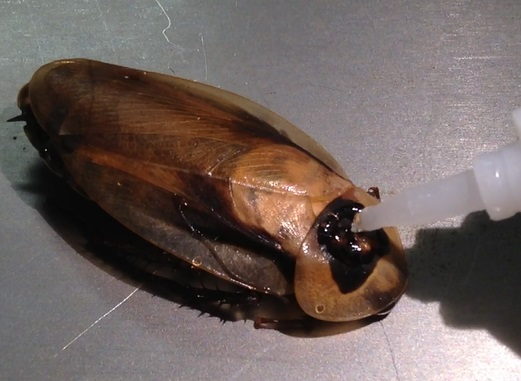
\includegraphics[scale=0.25]{Surgery Photos/gluepronotum.jpg}
\caption{Dab of glue on the pronotum}
\label{fig:gluepronotum}
\end{figure}
    
\item With the electrodes facing towards the antennae, gently place the black connector on the glue, orienting it squarely with the body so that the pins are parallel to the length of the body.
\begin{figure}[ht!]
\centering
    \begin{subfigure}{.4\textwidth}
    \centering
    \includegraphics[scale=0.3]{Surgery Photos/connector1.JPG}
    \caption{Square black connector}
    \label{fig:connector1}
    \end{subfigure}
    \begin{subfigure}{.4\textwidth}
    \centering
    \includegraphics[scale=0.3]{Surgery Photos/connector2.JPG}
    \caption{Place connector on glue dab}
    \label{fig:connector2}
    \end{subfigure}
\caption{Placing the black connector}
\label{fig:connector}
\end{figure}

\item After waiting \SIrange{1}{2}{\minute} for the glue to bond to the black connector,  place the roach back into the ice water for \SIrange{1}{2}{\minute}, ensuring that it is still anesthetized.
\end{enumerate}






\subsection{Implant the ground electrode}
\begin{enumerate}
\item Remove the cockroach from the ice water and place it on the table, belly down.
\item Carefully splay its right wing to the side, using silly putty to hold the wing down and stabilize it.
\begin{figure}[ht!]
\centering
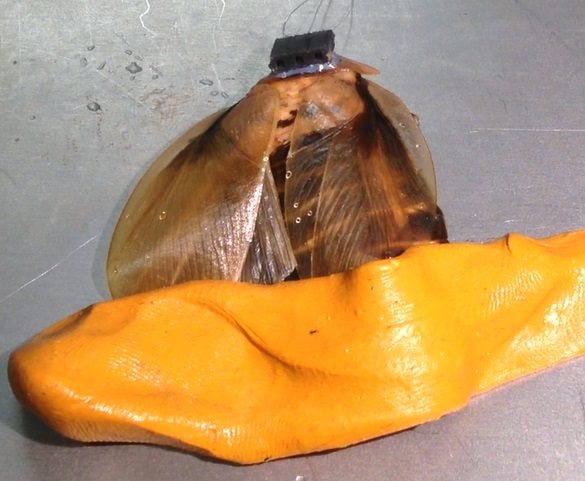
\includegraphics[scale=0.25]{Surgery Photos/putty.jpg}
\caption{Hold the wing down}
\label{fig:putty}
\end{figure}

\item Using a cotton swab, dry its thorax and then lightly sand the thorax in preparation for glue.
\item Using the needle and carefully keeping away from the center line to avoid the esophagus, lightly poke a small hole in the exoskeleton of the thorax, just behind its head.
\begin{figure}[ht!]
\centering
\includegraphics[scale=0.5]{Surgery Photos/avoidesoph.jpg}
\caption{Avoid the esophagus}
\label{fig:avoidesoph}
\end{figure}

	\subitem  If the roach has ``freckles'' on its back, use one of these as a reference for insertion points, which will make it easier to locate the hole when implanting the electrode.
	\begin{figure}[ht!]
	\centering
	\includegraphics[scale=0.3]{Surgery Photos/hole.jpg}
	\caption{Poke hole here}
	\label{fig:hole}
	\end{figure}

\item Using the fine forceps (tweezers), straighten the center electrode as much as possible and then carefully insert the electrode \SI{1}{\milli\meter} into the hole.
\begin{figure}[ht!]
\centering
\includegraphics[scale=0.4]{Surgery Photos/celectrode1.jpg}
\caption{Insert the center electrode}
\label{fig:celectrode1}
\end{figure}
 
\item  With a toothpick, apply a small bead of super glue to the electrode, just above where it entered the tissue.
\item Use the forceps to insert the electrode \SIrange{1}{3}{\milli\meter} into the hole, allowing the superglue to enter the body so that it will polymerize quickly and securely upon coming in contact with the internal saline.
{\begin{figure}[ht!]
\centering
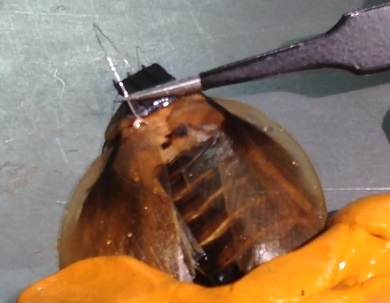
\includegraphics[scale=0.4]{Surgery Photos/celectrode2.jpg}
\caption{Insert the center electrode further}
\label{fig:celectrode2}
\end{figure}}
\item Replace the right wing to its resting place and allow the glue to set.
\item Once it has set, lightly tug to test if the ground electrode is secure.
\item Return the cockroach to the ice water for \SIrange{1}{2}{\minute} to maintain anesthetization.
\end{enumerate}










\subsubsection{Implant the right antenna electrode}
\begin{enumerate}
\item Take the roach out of the ice water and lay it on its back.
\begin{figure}[ht!]
\centering
\includegraphics[scale=0.3]{Surgery Photos/cut.jpg}
\caption{Cut the right antenna}
\label{fig:cut}
\end{figure}

\item Using the forceps to carefully splay the antenna out, cut the cockroach's right antenna to \SIrange{3}{6}{\milli\meter}.
\item Insert the right electrode \SI{1}{\milli\meter} inside the right antenna, not all the way in.
\begin{figure}[ht!]
\centering
\includegraphics[scale=0.3]{Surgery Photos/relectrode1.jpg}
\caption{Insert the right electrode}
\label{fig:relectrode1}
\end{figure}

\item Dab a bead of super glue just above where the electrode is in the antenna.
{\begin{figure}[ht!]
\centering
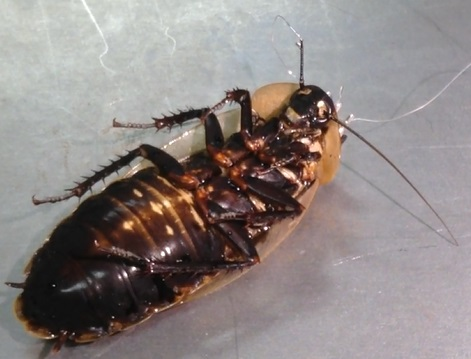
\includegraphics[scale=0.3]{Surgery Photos/relectrodeglue.jpg}
\caption{Apply a dab of glue}
\label{fig:relectrodeglue}
\end{figure}}

\item  Use the forceps to insert the electrode so that the bead of glue partially enters \SIrange{2}{4}{\milli\meter} into the antenna.
\subitem The goal is to get the glue just inside the inner ring of the antenna so the electrode will not fall out easily.
\begin{figure}[ht!]
\centering
\includegraphics[scale=0.3]{Surgery Photos/relectrode2.jpg}
\caption{Insert the right electrode further}
\label{fig:relectrode2}
\end{figure}

\item Put the roach back into the ice water for \SIrange{1}{2}{\minute} to maintain anesthetization.
\end{enumerate}






\subsubsection{Implant the left antenna electrode}
This section is the reverse of the previous. The cockroach should look like \fref{fig:lelectrode}.
\begin{figure}[ht!]
\centering
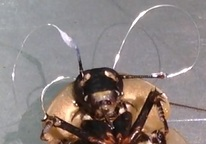
\includegraphics[scale=0.7]{Surgery Photos/lelectrode.jpg}
\caption{All electrodes in}
\label{fig:lelectrode}
\end{figure}
\begin{enumerate}
\item Take the roach out of the ice water and lay it on its back.
\item Using the forces to carefully splay the antenna out, cut the cockroach's left antenna to \SIrange{3}{6}{\milli\meter}.
\item Insert the left electrode \SI{1}{\milli\meter} inside the left antenna, not all the way in.
\item Dab a bead of super glue just above where the electrode is in the antenna.
\item Use the forceps to insert the electrode so that the bead of glue partially enters \SIrange{2}{4}{\milli\meter} into the antenna.
	\subitem The goal is to get the glue just inside the inner ring of the antenna so the electrode will not fall out easily.
\item Put the roach back into the ice water for \SIrange{1}{2}{\minute} to maintain anesthetization.
\end{enumerate}
      
      
      
      
      
      
      
\subsection{Tighten wire slack}
Because cockroach legs are strong and can pull the electrodes out if they get snagged, it is important to tighten the wire slack. 
\begin{figure}[ht!]
\centering
    \begin{subfigure}{.49\textwidth}
    \centering
    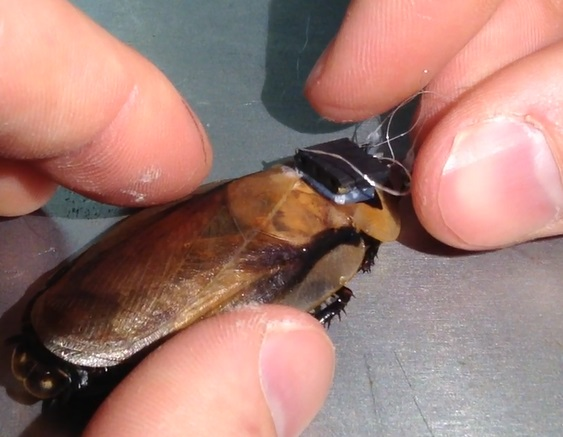
\includegraphics[scale=0.25]{Surgery Photos/nowire.JPG}
    \caption{Fold the wire slack}
    \label{fig:nowire}
    \end{subfigure}
    \begin{subfigure}{.49\textwidth}
    \centering
    \includegraphics[scale=0.4]{Surgery Photos/nowire2.JPG}
    \caption{Minimize wire slack}
    \label{fig:nowire2}
    \end{subfigure}
\caption{Tighten wire slack}
\label{fig:connectorB}
\end{figure}
\begin{enumerate}
\item Using the forceps and my fingers, carefully fold back the wire slack on top of the connector, trying to minimize the amount of slack wire between the antenna and connector. The exposed parts of silver wire cannot touch.
\item Wet and then dip the end of the popsicle stick in flour.
\item In order to hold the excess wire in place, take the glue gun and place a dab of hot glue on the wires, quickly using the flour end of the popsicle stick to smush down the glue.
\item Make sure that all the wires are tidy on the header, and apply extra glue to secure loose portions if necessary.
\end{enumerate}
\begin{figure}[ht!]
\centering
    \begin{subfigure}{.49\textwidth}
    \centering
    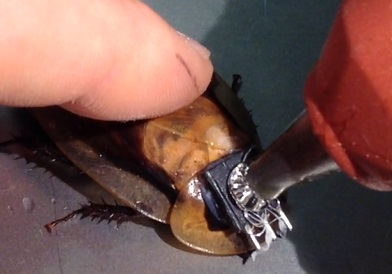
\includegraphics[scale=0.4]{Surgery Photos/gluewires.jpg}
    \caption{Apply a dab of hot glue}
    \label{fig:gluewires}
    \end{subfigure}
    \begin{subfigure}{.49\textwidth}
    \centering
    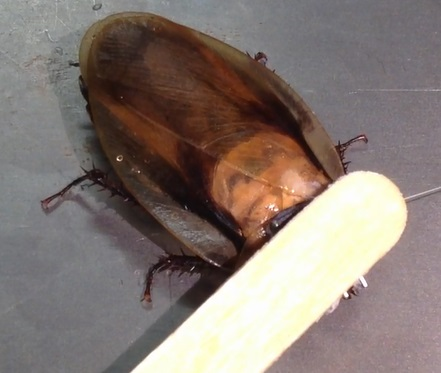
\includegraphics[scale=0.3]{Surgery Photos/gluewires1.jpg}
    \caption{Mash with the popsicle stick}
    \label{fig:gluewires1}
    \end{subfigure}
    \begin{subfigure}{.49\textwidth}
    \centering
    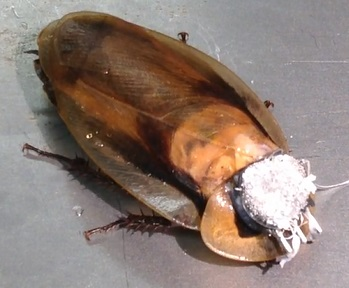
\includegraphics[scale=0.4]{Surgery Photos/gluewires2.jpg}
    \caption{Final product}
    \label{fig:gluewires2}
    \end{subfigure}
\caption{Glue the wires together}
\label{fig:connectorC}
\end{figure}







\subsection{End of surgery}
Once the surgery is complete, place the roach back in its terrarium, giving it at least \SIrange{2}{4}{\hour} if not a full night to recover. This surgery will be repeated for each cockroach participating in the experiment.
